%%%%%%%%%%%%%%%%%%%%%%%%%%%%%%%%%%%%%%%%%
% University/School Laboratory Report
% LaTeX Template
% Version 3.1 (25/3/14)
%
% This template has been downloaded from:
% http://www.LaTeXTemplates.com
%
% Original author:
% Linux and Unix Users Group at Virginia Tech Wiki 
% (https://vtluug.org/wiki/Example_LaTeX_chem_lab_report)
%
% License:
% CC BY-NC-SA 3.0 (http://creativecommons.org/licenses/by-nc-sa/3.0/)
%
%%%%%%%%%%%%%%%%%%%%%%%%%%%%%%%%%%%%%%%%%

%----------------------------------------------------------------------------------------
%	PACKAGES AND DOCUMENT CONFIGURATIONS
%----------------------------------------------------------------------------------------

\documentclass{article}

\usepackage{graphicx} % Required for the inclusion of images
\usepackage{amsmath} % Required for some math elements 
\usepackage{enumitem}
\usepackage{hyperref}
\usepackage[left=20mm,right=20mm,top=25mm,bottom=25mm]{geometry}
\usepackage{makecell}
\usepackage{float}

\title{Report: \textbf{University Rankings}} % Title

\author{Julian \textsc{Backé} \\ Tobias \textsc{Salzer} \\ Ajayvir \textsc{Singh}} % Author name


\begin{document}

\maketitle % Insert the title, author and date

In this work, we answer the following questions:

\begin{itemize}
	\item How do university rankings change over time? 
	
	\item Which characteristics of universities contribute most to good rankings, or to large changes in the ranking position? 
	
	\item How do these characteristics correlate with characteristics of cities or countries in which the university is located? 
	
	\item Are there predictors for increases or decreases in the rankings?
\end{itemize}

\section*{\large{How do university rankings change over time?}}
We obtained that the majority of universities have a rather stable ranking. This means that for most universities there are no huge changes in the rankings. However, there are also some (few) universities that jump in the rankings.

\section*{\large{Which characteristics of universities contribute most to good rankings, or to large changes in the ranking position?}}

For each survey, there are different characteristics contributing to the university rankings.

For the times survey, we were able to predict the scores and therefore also the rankings with pretty good accuracy. As input features for our model we used number of students, student-staff-ratio, percentage of international students and percentage of female students.

For the CWUR dataset, the resulting rank of a country is a transformation of other characteristics contained in the dataset, such as broad impact, publications, alumn employment, etc..
The exact methodology of these characteristics can be found \href{https://cwur.org/methodology/world-university-rankings.php}{ \textbf{here}}.
Consequently, it made sense to analyse which of these characteristics contribute most to good rankings. 
We were able to conclude, that the characteristics broad impact, publications and influence were among the top characteristics to contribute to good rankings, even though they were weighted the least, as mentioned in the above linked methodology.



\section*{\large{How do these characteristics correlate with characteristics of cities or countries in which the university is located?}}

The results of this section are summed up in Figure 1. For example, we obtained that a country's expenditure on education (in percent of the GDP) leads to a higher mean score of this country's universities (see Figure 2). However, a country's expenditures is not indicator on how good its best university will rank. We also found out that the number of universities per inhabitant as well as the Human Development Index (HDI) could be indicators for how good a country's universities will perform on average in rankings. It should be noted that with these characteristics it is possible to distinguish the mean ranks of different countries, but it is not possible to separate good and bad universities within the very same country

\begin{figure}[H]
\caption{Which local properties influence a country's university scores?}
\begin{center}
\begin{tabular}{|c|c|c|} \hline
\textbf{independent variable} & \textbf{dependent variable} & \textbf{impact} \\ \hline
\makecell{expenditures for education \\ (all institutions)} & mean score of country & YES \\ \hline
\makecell{expenditures for education \\ (all institutions)} & max. score of country & NO \\ \hline
\makecell{expenditures for education \\ (higher institutions)} & mean score of country & YES \\ \hline
\makecell{expenditures for education \\ (higher institutions)} & max. score of country & NO \\ \hline
\makecell{number of universities} & mean score of country & SLIGHT \\ \hline
\makecell{number of inhabitants} & mean score of country & NO \\ \hline
\makecell{univerisites per inhabitant} & mean score of country & YES \\ \hline
\makecell{HDI} & mean score of country & YES \\ \hline
\makecell{corruption} & mean score of country & todo \\ \hline
\end{tabular}
\end{center}
\end{figure}
\begin{figure}[H]
	\centering
	\caption{The influence of educational expenditure (in percentage of GDP) on university scores}
	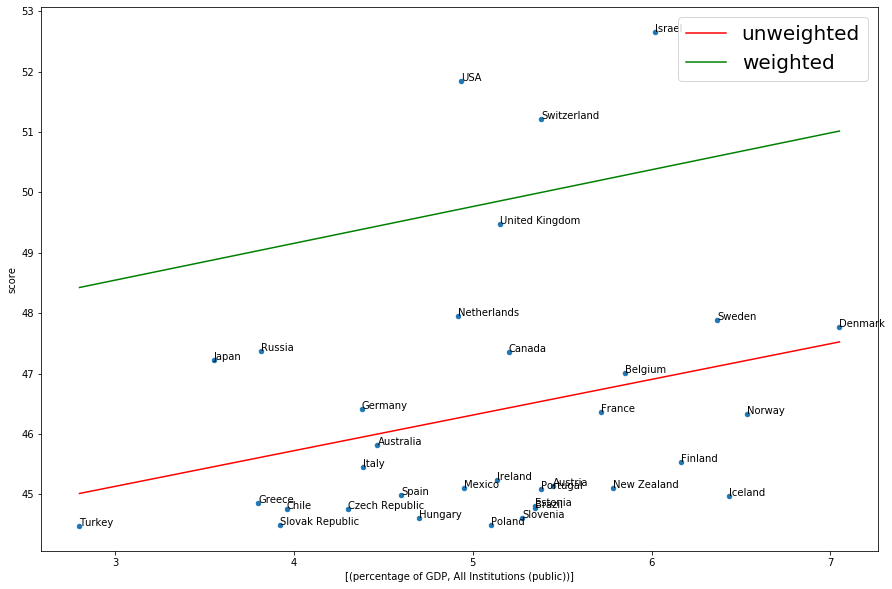
\includegraphics[width=0.75\linewidth]{graphs/exp_mean_all}
	
\end{figure}

\section*{\large{Are there predictors for increases or decreases in the rankings?}}
We constructed two models predicting a university's score: 

For one we considered some inherent characteristics of the university: number of students, the student staff ratio, the percentage of female students and the percentage of international students. For this model the Random Forest algorithm was used. In our tests, our model an average error of 3.38 score points, which implies a rather good model. 

For the second model, we calculated the mean rank by country, in an attempt to predict the average rank of a country, given the country's HDI. Using HDI as input, it was possible to construct a model within an error of 1.46 score. But it can be argued that the model struggles in predicting the actual ranks, and is more of an indicator of how well all universities of a country fare, given its HDI.





\end{document}